\section{Results}
\label{sec:results}

The operating point used throughout is
$k_xd=0.7362$, $k_yd=0.1298$, $\omega=7.6334\,c_s/d$, i.e.\
$f=\SI{16.68}{\giga\hertz}$ for $d=\SI{200}{\nano\metre}$, with the coupling
set to zero unless a sweep says otherwise, and with grounded faces.  The
reference plane for every reported return is $L=10\,d=\SI{2}{\micro\metre}$ from
the edge.  Unless stated otherwise the Galerkin degree is $n=22$.

\subsection{Dispersion and wave speeds}
\label{sec:results_dispersion}

\Cref{fig:fig01} characterises the guided branch that is later scattered at the
edge.  Panel (a) plots the frequency against $k_xd$ for the five coupling
levels.  The five curves superimpose to within the width of the line over the
whole range $0.15\le k_xd\le1.05$, and the inset resolves their difference: the
coupling lowers the frequency by at most \SI{184}{\kilo\hertz}, at
$k_xd=1.05$ where the carrier is \SI{16.87}{\giga\hertz}, that is by
$1.1\times10^{-5}$ in relative terms; at the negative coupling the lowering
stays below \SI{92}{\kilo\hertz} over the same range.  This is the first indication, confirmed in \cref{sec:results_coupling},
that the added coupling is a perturbation of the dispersion and a modifier of
the edge partition rather than a driver of the branch itself.

Panel (b) separates three velocities that must not be confused:
\begin{align}
v_p&=\frac{\omega}{|\vect{k}|}=\frac{\omega}{\sqrt{k_x^2+k_y^2}},
\qquad \text{(phase speed, a magnitude)}\label{eq:vp}\\
v_g&=c_s\frac{\partial\omega}{\partial k_x},
\qquad \text{(group velocity, signed)}\label{eq:vg}\\
v_E&=\frac{\mathcal{P}_x}{E},
\qquad \text{(energy velocity, signed)}\label{eq:vE}
\end{align}
with $\mathcal{P}_x$ from \eqref{eq:Px_int} and $E$ the stored energy per unit
length.  The phase speed \eqref{eq:vp} is a positive magnitude and cannot
change sign; it is plotted on the right-hand axis of panel (b) and it decreases
monotonically from \SI{105.8}{\kilo\metre\per\second} at $k_xd=1.05$ to
\SI{20.0}{\kilo\metre\per\second} near the cutoff, as a phase speed should.  The
group and energy velocities are signed and are plotted on the left-hand axis:
they run from $-188$ and $-189$ to $+1097$ and $+1136\,\si{\metre\per\second}$,
change sign just below $k_xd=0.53$, and agree with each other to within
\SI{3.5}{\percent} at every sample except the lowest, where the two differ by
\SI{6.4}{\percent} because both velocities pass close to zero there.  The sign change of $v_g$ and $v_E$ marks the backward part of the branch.  A
backward branch exists whether or not an edge is present, and what the edge adds
is the conversion into it: the branch provides a mode whose energy travels
opposite to the phase, and that is the mode the edge subsequently selects.

Panels (c) and (d) report the linewidth and the attenuation.  The linewidth
ranges from \SI{1.4}{\kilo\hertz} to \SI{0.27}{\mega\hertz} and grows
monotonically with $k_xd$, with a clear ordering in $H$.  The attenuation
$\alpha=2|\Imag k_x|$, obtained from the complex spatial root at real frequency,
ranges from \SI{0.23}{\deci\bel\per\milli\metre} to
\SI{456}{\deci\bel\per\milli\metre}, peaks sharply at $k_xd\approx0.52$ and is
positive everywhere on the branch.

\begin{figure}[htbp]
\centering
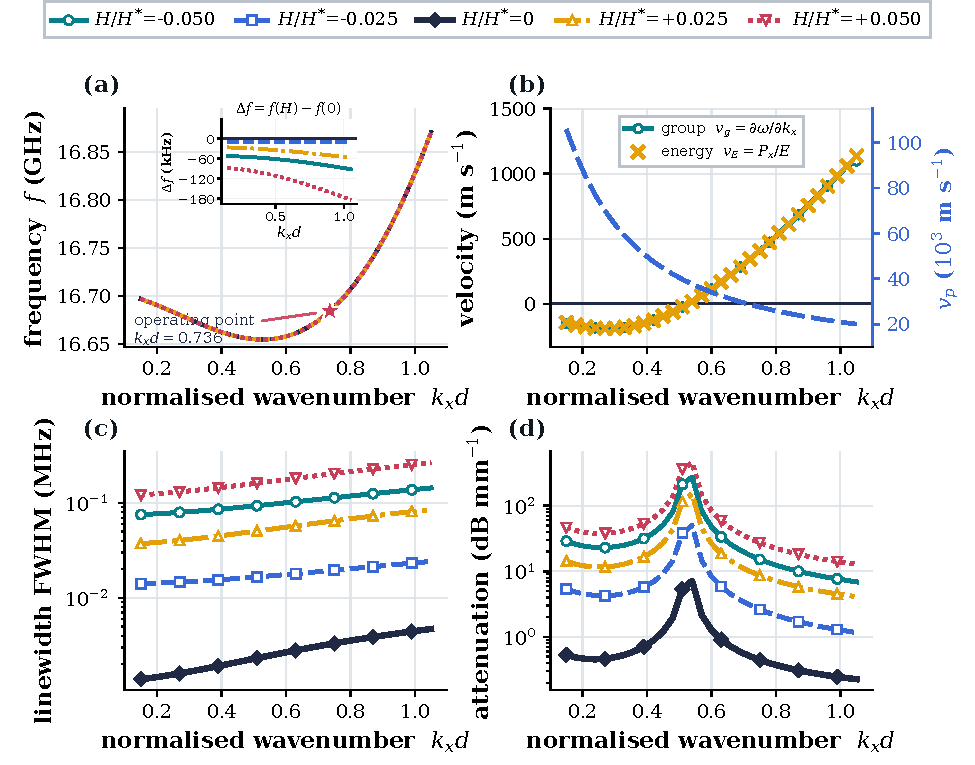
\includegraphics[width=0.95\textwidth]{figures/fig01_dispersion.pdf}
\caption{Dispersion and wave speeds of the guided branch.  (a) Frequency against
$k_xd$ for five coupling levels; the five curves coincide and the inset resolves
$\Delta f=f(H)-f(0)$ in kHz, with the operating point $k_xd=0.736$ marked.
(b) Group and energy velocities (left axis, signed) and phase speed (right axis,
a magnitude) at $H=0$; $v_g$ and $v_E$ change sign just below $k_xd=0.53$
while $v_p$ does not.  (c) Linewidth and (d) attenuation
$\alpha=2|\Imag k_x|$ for the same five levels, at
$d=\SI{200}{\nano\metre}$ and $n_0=\SI{2e18}{\per\cubic\metre}$.}
\label{fig:fig01}
\end{figure}

\subsection{The material specialisation and the role of the flexoelectric sector}
\label{sec:results_scope}

The title names the full flexoelectric framework, and it is worth fixing which
part of \eqref{eq:enthalpy} the calculations exercise before the numbers are
read.

Four sectors are active in every solve: the elastic, the strain-gradient, the
piezoelectric and the carrier sector.  The flexoelectric sector is active but
subdominant.  A single flexoelectric constant $f\equiv f_{3zz}=\SI{1}{\nano
\coulomb\per\metre}$ is retained --- a value at the low end of the range
reported for ZnO, and synthetic in the sense that it is not a measurement on the
crystal used for the elastic constants --- which gives the dimensionless
coupling $f=2.56\times10^{-3}$ of \cref{tab:groups}.  The added
carrier--strain-gradient coupling is swept over
$|H|\le\SI{2.0e-23}{\joule\metre}=0.022\,H_{\text{bound}}$, i.e.\ over the
range allowed by \eqref{eq:schur}.

The contribution of the flexoelectric term was measured rather than assumed, by
repeating the two solved configurations with $f$ set to zero and to ten times
the retained value (part of the study reported in \cref{tab:controls}).  At the
operating point the backward
channel is $0.0231456$ with the retained $f$ and $0.0231484$ with $f=0$, a
change of \SI{-0.012}{\percent}; at $k_xd=0.55$ it is $0.579180$ and
$0.579245$, a change of \SI{-0.011}{\percent}.  At ten times the retained value the changes
are \SI{-1.20}{\percent} and \SI{-1.12}{\percent}, so the dependence is smooth
and linear in the coupling rather than a threshold effect.

Read together, these numbers place the reported returns at one part in ten
thousand of the returns of the \emph{strain-gradient
piezoelectric-semiconductor} specialisation with the added carrier coupling.
The flexoelectric term is present and contributes with the correct sign and
magnitude, and it does not drive the effect.  What the numbers support is a
slow-mode edge effect of the strain-gradient plate, modulated by the carrier
coupling, inside a flexoelectric-semiconductor formulation; they do not support
the attribution of the negative reflection to the flexoelectric mechanism
itself.

\subsection{Carrier density and mobility}
\label{sec:results_material}

\Cref{fig:fig02} sweeps the two material families.  Increasing the carrier
density from $1$ to $3\times10^{18}\,\si{\per\cubic\metre}$ raises the linewidth
(a) and the attenuation (b) by roughly a factor of nine and a factor of ten
respectively, and lowers the frequency only slightly.  Panel (c) is the
important one: the backward channel at the reference plane is plotted against
$k_xd$ for the five densities, and the five curves collapse onto one.  The
maximum of $R_B=0.5796$ is reached near $k_xd=0.55$ for every density, and the
relative spread between the five curves is below \SI{0.2}{\percent} over the
whole range.  The carrier density therefore sets the loss and the dispersion
margin but not the partition of the scattered power.

The mobility behaves in the same way (panel d): over the factor-of-three range
$0.00875$ to $0.02625\,\si{\square\metre\per\volt\per\second}$ the linewidth
changes by a factor of about five while the reflectance is unchanged to the
same $0.2$ per cent.  Both results are consistent with $Q=d/L_D=0.075<1$: the
plate is thinner than the Debye length, the carrier perturbation is not confined
to a surface layer, and the density enters the problem mainly through the
conduction loss.

Every row of this sweep satisfies the conservation bound \eqref{eq:admissible}; the curve in panel (c) extends to $k_xd=0.9$ and falls to
$10^{-7}$ there, which is the backward port ceasing to carry energy rather than
a numerical failure.  Rows at that end have $|\cos\theta_E|\to0$, and the flux
fraction is stored with each row so that the loss of resolution is visible.

\begin{figure}[htbp]
\centering
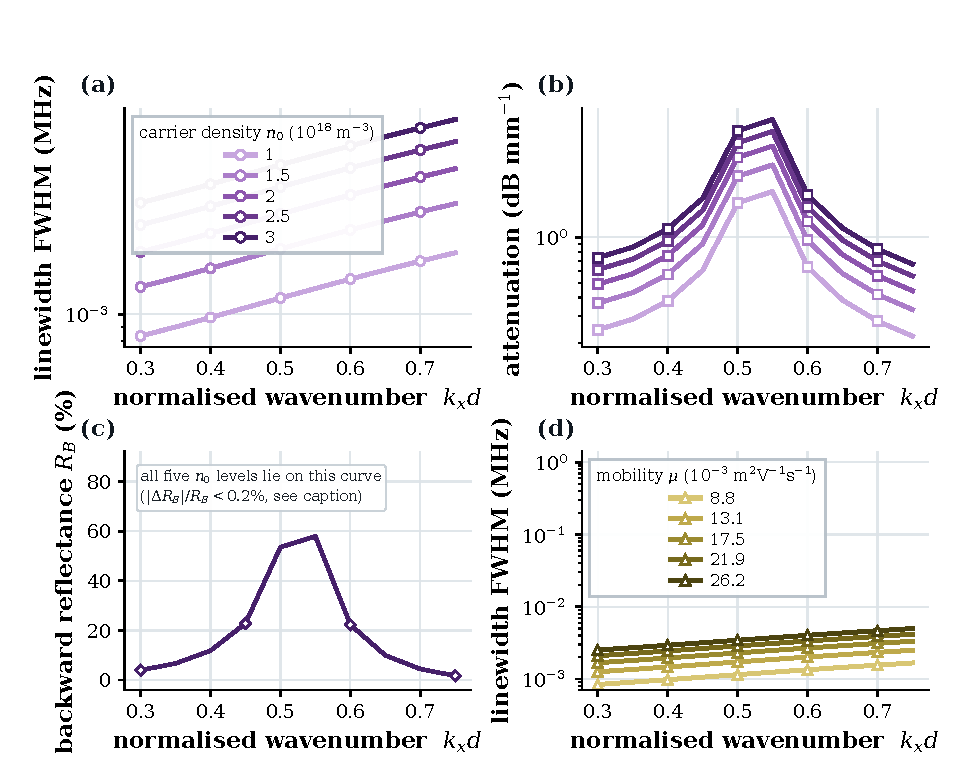
\includegraphics[width=0.95\textwidth]{figures/fig02_material.pdf}
\caption{Carrier density and mobility.  (a) Linewidth and (b) attenuation against $k_xd$ for five carrier densities
$n_0=1\ldots3\times10^{18}\,\si{\per\cubic\metre}$; (c) the backward share at
the reference plane $L=\SI{2}{\micro\metre}$, independent of the density to
within \SI{0.2}{\percent}, with its largest sampled value $R_B=0.5796$ at
$k_xd=0.55$; (d) linewidth for five mobilities.}
\label{fig:fig02}
\end{figure}

\subsection{Thickness and gradient length}
\label{sec:results_geometry}

\Cref{fig:fig03} separates the two geometric families, which scale differently
and must not be plotted on a common axis.  Plate thickness is the dominant
scale: between \SI{120}{\nano\metre} and \SI{320}{\nano\metre} the branch moves
from \SI{30.4}{\giga\hertz} to \SI{10.5}{\giga\hertz} and the relative change is
of order unity for every wavenumber (panels a and c).  The gradient length is a
weak perturbation of the same branch (panels b and d): relative to
$\ell=\SI{50}{\nano\metre}$, a change to $\ell=\SI{90}{\nano\metre}$ shifts the
frequency by \SI{+2.0}{\percent} at $k_xd=0.15$ and by \SI{+10.2}{\percent} at
$k_xd=1.05$, while $\ell=\SI{35}{\nano\metre}$ shifts it by \SI{-1.9}{\percent}
and \SI{-4.9}{\percent} at the same two points.  The sign of the effect changes
with $\ell$ across the reference value, which is why the panel is plotted as a
relative change and not as an absolute frequency.

The distinction matters for the interpretation of the rest of the paper.  A
thickness change rescales the whole problem and is not a coupling effect; a
gradient-length change alters the relative weight of the hyperelastic and
flexoelectric terms at fixed geometry and is therefore the parameter that
belongs with $H$ in a discussion of the added physics.

\begin{figure}[htbp]
\centering
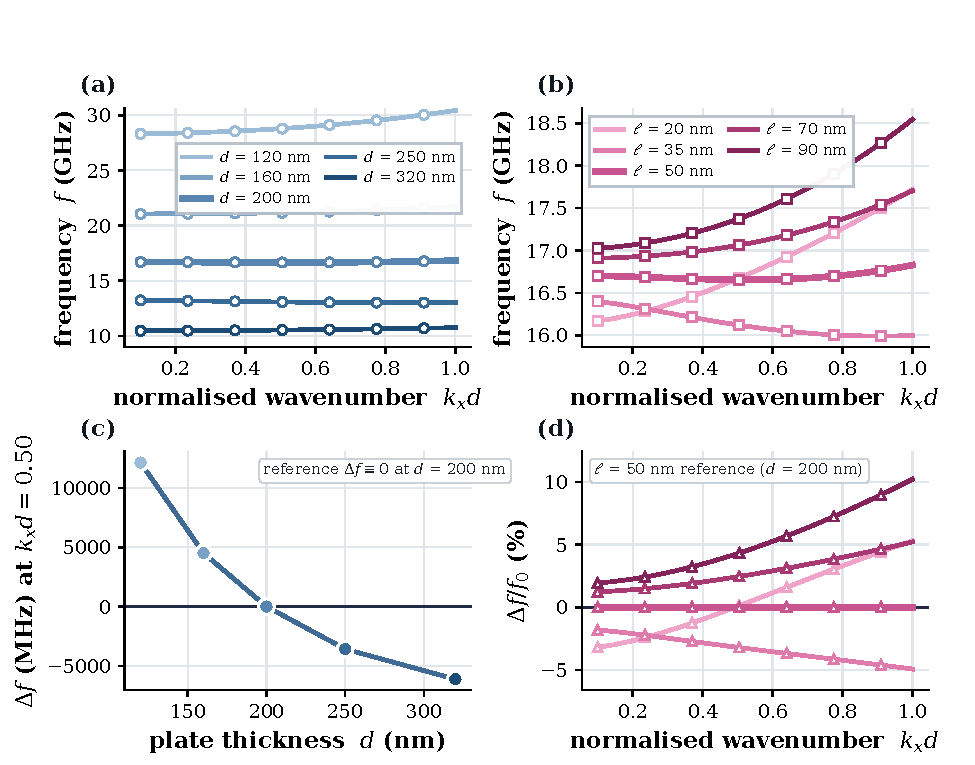
\includegraphics[width=0.95\textwidth]{figures/fig03_geometry.pdf}
\caption{Plate thickness and gradient length, kept as separate families.
(a) Dispersion for five thicknesses at $\ell=\SI{50}{\nano\metre}$;
(b) dispersion for five gradient lengths at $d=\SI{200}{\nano\metre}$;
(c) $\Delta f$ at $k_xd=0.50$ against thickness, with the reference
$\Delta f\equiv0$ at $d=\SI{200}{\nano\metre}$; (d) relative frequency change
against $k_xd$ for the five gradient lengths.}
\label{fig:fig03}
\end{figure}

\subsection{Backward conversion along the branch}
\label{sec:results_frequency}

\Cref{fig:fig04} sweeps the drive along the solved guided branch rather than at
a fixed frequency.  The distinction matters away from the operating point, where
a fixed-frequency solve does not return the physical continuation of the branch
and the energy angle collapses towards $-90^{\circ}$; following the branch gives,
for every row, a resolved triple of frequency, wavenumber and return.  Two
rasters are used: a coarse one over the whole window and, at $H=0$ only, a fine
one of spacing $\Delta k_xd=5\times10^{-4}$ across $0.520\le k_xd\le0.535$,
because the top of the response is three orders of magnitude narrower than any
raster that can be drawn on a single axis.  The number of rows is a property of
the grid and is recorded with the data.

The share along the branch is largest on its slow part.  It is $0.0399$
at $k_xd=0.30$ ($f=\SI{16.676}{\giga\hertz}$), rises to $0.9468$ at
$k_xd=0.5275$ ($f=\SI{16.6547}{\giga\hertz}$), and falls to $0.0173$ at
$k_xd=0.75$ ($f=\SI{16.688}{\giga\hertz}$) (panel a).  The response is
single-humped over the whole window: the coarse raster finds no second local
extremum, and the top of the hump is located in
\cref{sec:results_certification}.  Panel (b) shows the signed energy angle
changing by $16^{\circ}$ across the window and passing through its own extremum
beside the maximum of $R_B$, so the two are not independent readings.  Panel (c)
plots the same data against the ratio $k_{Bx}/k_{ix}$: all five coupling levels
collapse onto one master curve, and the conversion is largest where the backward
wavenumber approaches the incident one, reaching $k_{Bx}/k_{ix}=0.9960$ at the
maximum.  The backward port is therefore a genuine propagating mode of the
higher-order branch, not an evanescent artefact, and the projection onto it
becomes decisive exactly where the two wavenumbers approach each other.  Panel
(d) shows why they do: the branch passes through a zero-group-velocity point at
$k_xd\approx0.527$, where $|v_g|$ falls below \SI{1}{\metre\per\second} against
$-180$ and $+355\,\si{\metre\per\second}$ at the two ends of the window, and the
incident and backward wavenumbers close on one another there and open again
beyond it.

\begin{figure}[htbp]
\centering
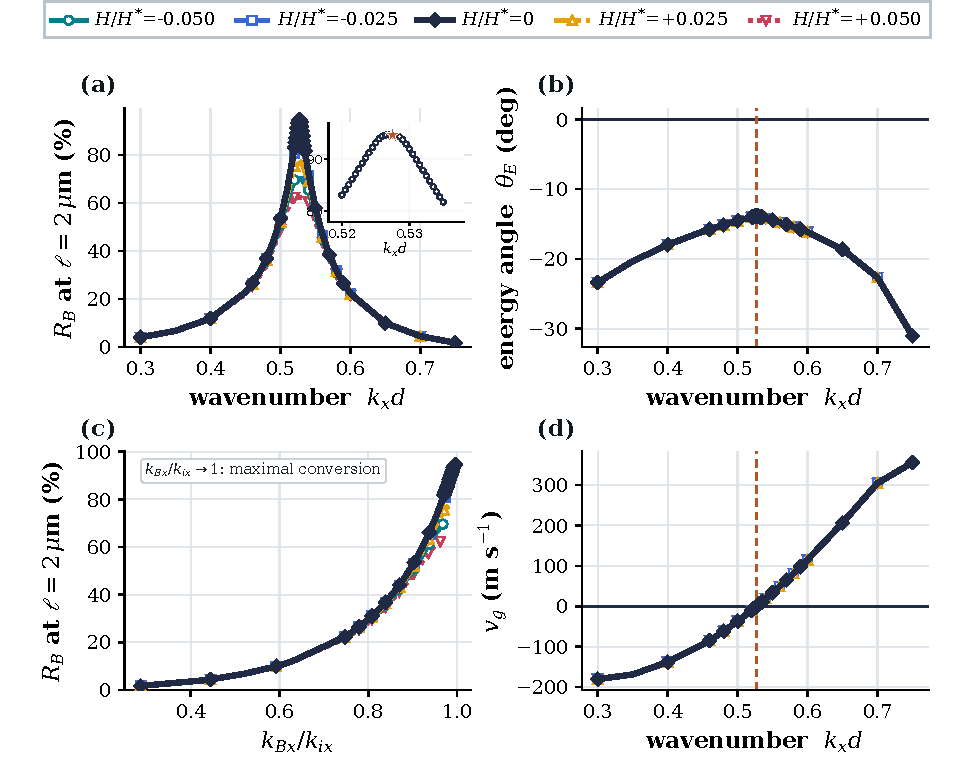
\includegraphics[width=0.95\textwidth]{figures/fig04_frequency.pdf}
\caption{Backward conversion along the guided branch; every plotted row
satisfies the conservation bound \eqref{eq:admissible}.  (a) Backward channel
against the wavenumber, with the maximum of the $H=0$ branch marked by
a star and its top resolved in the inset on the same data; (b) signed energy
angle; (c) backward channel against the wavenumber ratio $k_{Bx}/k_{ix}$;
(d) group velocity, with the dashed line at the maximum.  The five
coupling levels are drawn in every panel.  The top of the response is resolved in the inset, which uses the same data.}
\label{fig:fig04}
\end{figure}

\subsection{Convergence of the reported values}
\label{sec:results_peak}

The maximum of \cref{fig:fig04} falls between two samples of the coarse raster,
so it is solved again at four Galerkin degrees with the same physics, and each
value is checked against the quadrature rule.  \Cref{tab:refinement} reports the
outcome.

\begin{table}[t]
\centering
\caption{Refinement of the reported values with the Galerkin degree $n$.  The
last column is the largest relative change of $R_B$ with respect to the
degree-30 value.  All four configurations use the same physics, the same
reference plane and $H=0$.}
\label{tab:refinement}
\begin{tabular}{@{}lcccc@{}}
\toprule
Case & $k_xd$ & $R_B$ at $n=30$ & $\theta_E$ at $n=30$ (deg) & $\max|\Delta R_B|/R_B$ \\
\midrule
Operating point   & 0.7362 & 0.023\,146 & $-27.8997$ & $7.2\times10^{-7}$ \\
Maximum & 0.5275 & 0.946\,795 & $-13.8506$ & $3.8\times10^{-9}$ \\
Earlier sample    & 0.5250 & 0.931\,891 & $-13.8888$ & $2.3\times10^{-8}$ \\
$k_xd=0.55$       & 0.5500 & 0.579\,180 & $-14.4487$ & $1.5\times10^{-7}$ \\
\bottomrule
\end{tabular}
\end{table}

Three properties of the sequence are worth recording.  First, the values are
converged in the Galerkin degree: between degrees 14 and 34 the relative
change of the maximum stays below $10^{-8}$ at both the located argmax and the
reported wavenumber, the operating point changes by $7.2\times10^{-7}$, and the
successive changes decrease monotonically, which is what a spectral method
should do.  The two spreads are differences of nearly equal numbers and lie on
the round-off floor, so they are quoted as bounds and not as values.  No rate is
fitted, because the sequence reaches that floor before an asymptotic slope
exists.  Quadrature is not a limitation either: with the degree fixed at 22 and
the rule taken from 64 to 256 nodes the maximum changes by less than $10^{-8}$.  Second, the values
are well conditioned: the singular-value condition number of the edge system is
at most $1.9\times10^{2}$ and the scaled edge residual is below
$3\times10^{-15}$ in every case.  Third, the values are resolved projections:
the energy angles are $-13.9^{\circ}$ and $-27.9^{\circ}$, so the measured $x$
flux is \SI{97.1}{\percent} and \SI{88.4}{\percent} of the total modal flux
respectively.  Neither value is an artefact of a near-grazing mode.

One sensitivity sets the precision of the printed digits.  The spatial problem
is solved at the real part of the tracked frequency, and on a flat branch that
map is ill-conditioned: a relative change of $1.8\times10^{-12}$ in the
frequency moves $R_B$ by $5.6\times10^{-6}$.  The maximum is therefore
reproducible to about $\pm6\times10^{-6}$ ($\pm0.0006$ percentage point) even
though the Galerkin and quadrature errors are two to three orders smaller.
Beyond that, the incident wavenumber returned by the spatial problem is
$k_{ix}d=0.52824$, not the branch parameter $k_xd=0.5275$: on a flat branch the
two differ by \SI{0.14}{\percent} at the maximum.  Both are tabulated and no
conclusion depends on the difference.

\subsection{Location of the maximum}
\label{sec:results_certification}

The quantity maximised is the one defined by \eqref{eq:RB}: the modal self-power
of the identified backward outgoing mode at the reference plane, divided by the
incident power at the same plane with the incident mode normalised to unity.
The other outgoing modes, the interference term and the dissipation are quoted
separately and are never folded into it; the edge-plane value is reported beside
the reference-plane value and never substituted for it.

The location is found in three stages.  A coarse raster of
$\Delta k_xd=0.002$ over $0.465\le k_xd\le0.625$ -- the whole window in which a
backward port exists at this $k_y$ -- contains a single hump and no second local
extremum, with its largest sample at $k_xd=0.527$.  A plateau raster of
$\Delta k_xd=10^{-4}$ over $0.5265\le k_xd\le0.5285$, and a refined raster of
$\Delta k_xd=10^{-5}$ over $0.5272\le k_xd\le0.5278$, place the maximum at
$k_xd=0.52752$ with $R_B=0.9467954$; the value at the reported wavenumber
$k_xd=0.5275$ is $R_B=0.9467952$, $1.4\times10^{-7}$ lower, which is below the
reproducibility of the frequency map.  Every sampled wavenumber in
$0.5266\le k_xd\le0.5277$ lies within \SI{0.01}{} percentage point of the
maximum and every sampled wavenumber in $0.5265\le k_xd\le0.5281$ within
\SI{0.1}{} percentage point, so the response has a flat top rather than a sharp
peak: the reported location is the centre of that top, determined to within its
half-width of $\pm0.0009$, not a five-digit abscissa.

Two independent restarts, from the brackets $[0.520,0.532]$ and
$[0.524,0.536]$ on a raster of $10^{-3}$, return the same interval and the same
sample value, $8.4\times10^{-6}$ below the refined maximum: the restarts test the
bracketing, not the refinement, which is what the two finer rasters above are
for.  The result is a \emph{local maximum within the declared window}.  It is not a
global maximum over all $k_y$, all thicknesses or all material sets, none of
which is searched here.  The search record also stores whether the refined
raster is flat and interior; a raster that is not flat, or that meets the
boundary of the interval, is reported as the largest sample rather than as a
maximum.

\subsection{The maximum read as a modal share}
\label{sec:results_artefact}

Three properties of the solution decide whether such a number can be read at
face value.

\emph{A small denominator.}  The incident flux at the maximum is small, a
factor $128$ below its value at the operating point, so the fraction could in
principle be a ratio of two nearly vanishing quantities.  It is not: the value
is reproduced to better than $10^{-8}$ across six Galerkin degrees, to
better than $10^{-8}$ across four quadrature rules, and identically along three
different tracking paths that reach the same wavenumber from below, from above
and in a single step.  A ratio of two independently vanishing numbers would
scatter under all three.

\emph{Which branch.}  The reference plane is moved from $0$ to $20$
thicknesses and the partition is rescaled by
$\exp[2(|\Imag k_{ix}|+|\Imag k_{Bx}|)(L-L_{\text{ref}})/d]$, which is the net
attenuation of the two partner modes travelling in opposite directions.  The
rescaled values agree to $2\times10^{-16}$, so the number is a property of the
edge and both attenuations are resolved rather than assumed.  The transform is
implemented once and imported everywhere it is used, and the stored edge-plane
fractions of the search, of the matched controls and of the coupling dataset
are reproduced by a fresh evaluation to $10^{-10}$ relative or better; the plane at
which a share is quoted is therefore a reporting choice and not a second
definition.  The backward port
is also unique: the second outgoing candidate lies $2.0|k_x|$ away, the
condition number of the normalised edge matrix is $1.6\times10^{2}$, and the
relative error bound of the projection is $\text{cond}\times\epsilon=4\times10^{-14}$.

\emph{Nearly parallel modes.}  The incident and backward eigenvectors
are nearly parallel, with overlap $0.999995$, and their wavenumbers are
separated by $1.45$ times the modal decay rate: close, but resolved.  The
partition rebuilt from the stored amplitudes and modal powers alone reproduces the computed value to machine precision, which is the direct statement that no
eigenvector phase or scale enters the result.  What the near-coincidence does
change is interpretation, not accuracy: because the incident flux falls towards
the fold, the fraction is anti-correlated with it across the window
($r=-0.96$), so a maximal share coexists with a minimal transported power.

The maximum is a modal share and not a reflectance.  At $k_xd=0.5275$ the
total outgoing propagating power is $0.99769$ of the incident power and the
interference correction at the reference plane is $-2.29\times10^{-3}$, so the
backward mode carries \SI{94.68}{\percent} of the incident power and
\SI{94.90}{\percent} of the outgoing propagating power.  The modal share is
\SI{94.68}{\percent}; the energy statement is that \SI{99.77}{\percent} leaves
as propagating outgoing modes.  The two are different readings of the same
solution.

The maximum must also be read with its own amplitude in mind.  It sits on a
zero-group-velocity fold, and a mode with vanishing group velocity carries
vanishing flux: the incident modal power per unit normalisation falls from
$5.08\times10^{-3}$ at the operating point to $3.97\times10^{-5}$ at the
maximum, a factor $128$, while $|\Imag k_{ix}|d$ rises to $1.0\times10^{-3}$.
The fraction is therefore the ratio of two small but resolved fluxes -- well
defined, unchanged by the incident normalisation, and stable to
$1\times10^{-8}$ under degree and quadrature refinement -- but it is not a statement that a
large amount of energy is turned around.  Both readings are needed: the
partition is maximal at the fold and the transported power is minimal there.

The three configurations are compared term by term in
\cref{tab:configurations}.  Every entry is evaluated at degree 30, except the
attenuations, which are $2|\Imag k_x|/d$ formed from the same spatial roots.

\begin{table}[t]
\centering
\caption{The three reported configurations.  All are solved with
$d=\SI{200}{\nano\metre}$, $n_0=\SI{2e18}{\per\cubic\metre}$,
$\ell=\SI{50}{\nano\metre}$, $H=0$, $k_yd=0.1298$, grounded faces and a
reference plane $L=10d=\SI{2}{\micro\metre}$ from the edge.  ``Isolated
backward return'' is the modal share \eqref{eq:RB}, with the incident
self-power normalised to unity; it is not a total reflectance.}
\label{tab:configurations}
\small
\begin{tabular}{@{}lccc@{}}
\toprule
Quantity & Operating point & Maximum & $k_xd=0.55$ \\
\midrule
frequency & $\SI{16.684}{\giga\hertz}$ & $\SI{16.6547}{\giga\hertz}$ & $\SI{16.6550}{\giga\hertz}$ \\
longitudinal wavenumber $k_xd$ & 0.7362 & 0.5275 & 0.5500 \\
incident wavenumber $\Real k_{ix}d$ & 0.7362 & 0.5282 & 0.5500 \\
group velocity $v_g$ & $\SI{0.37}{\kilo\metre\per\second}$ & $\SI{0.45}{\metre\per\second}$ & $\SI{0.034}{\kilo\metre\per\second}$ \\
incident attenuation $2|\Imag k_{ix}|$ & \SI{0.469}{\deci\bel\per\milli\metre} & \SI{87.2}{\deci\bel\per\milli\metre} & \SI{4.02}{\deci\bel\per\milli\metre} \\
backward attenuation $2|\Imag k_{Bx}|$ & \SI{0.454}{\deci\bel\per\milli\metre} & \SI{87.1}{\deci\bel\per\milli\metre} & \SI{3.93}{\deci\bel\per\milli\metre} \\
isolated backward return $R_B$ & $0.0231456$ & $0.9467952$ & $0.5791801$ \\
modal share at the edge plane & $0.0232$ & $0.9856$ & $0.5802$ \\
energy angle $\theta_E$ & $-27.90^{\circ}$ & $-13.85^{\circ}$ & $-14.45^{\circ}$ \\
total outgoing propagating power & $0.99980$ & $0.99769$ & $0.99881$ \\
interference $P_{\text{cross}}/P_{\text{inc}}$ & $-4.17\times10^{-6}$ & $-2.29\times10^{-3}$ & $-1.02\times10^{-3}$ \\
dissipation $P_{\text{diss}}/P_{\text{inc}}$ & $1.99\times10^{-4}$ & $2.32\times10^{-5}$ & $1.72\times10^{-4}$ \\
edge-system condition number & $1.86\times10^{2}$ & $1.86\times10^{2}$ & $1.86\times10^{2}$ \\
scaled edge residual & $\le3\times10^{-15}$ & $\le3\times10^{-15}$ & $\le3\times10^{-15}$ \\
\bottomrule
\end{tabular}
\end{table}

\subsection{Energy budget of the edge problem}
\label{sec:results_channel}

\Cref{fig:fig05} closes the energy identity \eqref{eq:energy_identity} at the
reference plane.  At $H=0$ the incident power normalised to unity is partitioned
as follows: the identified backward channel carries $2.3146\times10^{-2}$, the
remaining propagating outgoing modes carry $0.976651$, dissipation removes
$1.985\times10^{-4}$, and the interference term is $-4.169\times10^{-6}$.  As
rounded, these four numbers close to $1.4\times10^{-6}$; evaluated at full
precision the identity closes to $1.9\times10^{-17}$, and the computed power balance to $6.6\times10^{-13}$, six orders of magnitude below the $10^{-6}$
threshold plotted in panel (c).  At the maximum the partition is
$0.946795$ in the backward channel, $5.089\times10^{-2}$ in the remaining
propagating modes, $2.32\times10^{-5}$ dissipated and $-2.29\times10^{-3}$ in
the interference term, which sums to $0.99769$ against an incident power of
unity; the same identity closes to $3.0\times10^{-13}$.

The evanescent spectrum does not belong to the transported budget.  At the
reference plane the entire evanescent content has decayed by a factor
$\exp(-2|{\Imag k_x}|L)$ with $|{\Imag k_x}|L\gtrsim10$, which leaves
$4.8\times10^{-28}$ of the incident power.  Reactive bookkeeping is meaningful
only at the edge plane itself, where it is $4.4\times10^{-6}$, and even there it
is not transported energy.  For the same reason $P_{\text{cross}}$ is an
interference correction and not a channel, and the evanescent members of
$\{P_j\}$ are reactive; the complete statement is the partition above, with the
interference term quoted explicitly.

Panels (b) and (d) sweep the coupling at the \emph{fixed} operating frequency
$\omega=\omega_0$, so the incident wavenumber drifts with $H$ along the branch
instead of the frequency doing so.  That is the response of the plate driven at
one frequency; the branch-consistent comparison is the one in
\cref{tab:controls}.  At
fixed frequency the backward channel changes from $2.2865\times10^{-2}$ at
$H/H^{*}=-0.05$ to $2.2658\times10^{-2}$ at $H/H^{*}=+0.05$, a variation of
\SI{2.1}{\percent}; dissipation rises from $6.9\times10^{-3}$ to
$1.2\times10^{-2}$; the other propagating modes carry the balance.  Panel (d)
gives the same information as a relative change against the uncoupled baseline:
the largest deviation is \SI{-2.11}{\percent} at $H/H^{*}=+0.05$.  When instead
$k_x$ is held fixed and the frequency follows the branch --- the comparison that
\cref{tab:controls} performs --- the deviation at the same tabulated extreme is
\SI{-1.21}{\percent}: part of the fixed-frequency variation is the dispersion
shift of $H$, which is even in $H$ and reaches $6.3\times10^{-5}$ in $\omega$.

\begin{figure}[htbp]
\centering
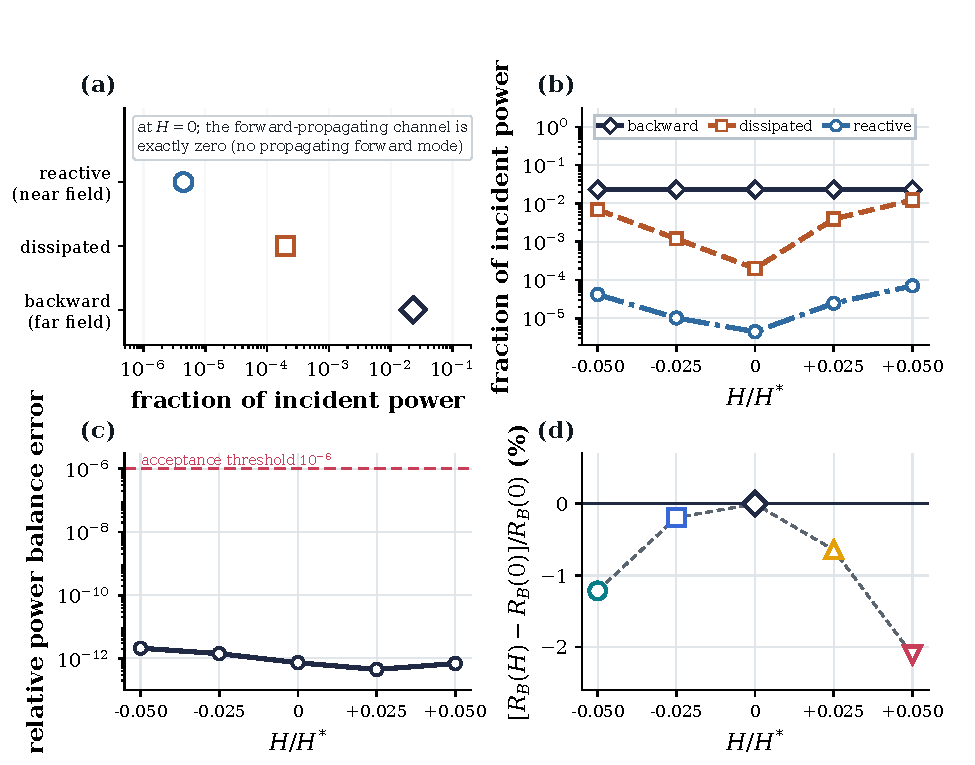
\includegraphics[width=0.95\textwidth]{figures/fig05_channel.pdf}
\caption{Complete energy budget at the reference plane $x=-2\,d$.  (a) Partition
of the incident power at $H=0$, logarithmic axis: backward channel
$2.31\times10^{-2}$, other propagating outgoing modes $0.976651$, dissipation
$1.99\times10^{-4}$, interference $|P_{\text{cross}}|=4.17\times10^{-6}$.
(b) The four fractions against $H/H^{*}$ at fixed operating frequency, so that
the incident wavenumber drifts with $H$; \cref{tab:controls} gives the
branch-consistent sweep.  (c) Relative power balance error with the $10^{-6}$
acceptance line.  (d) Relative change of the backward channel with respect to
$H=0$ at fixed frequency.}
\label{fig:fig05}
\end{figure}

\subsection{What creates the backward channel}
\label{sec:results_mechanism}

The partition quoted above was computed at $H=0$, with the
carrier--strain-gradient coupling switched off, and the contribution of that
coupling is isolated by matched controls: every ingredient except the named one
is held fixed (same $k_x$, same $k_y$, same $n_0$, same $\ell$, same reference
plane, same unit incident self-power), and the frequency follows the branch,
because switching an ingredient off changes the dispersion and solutions taken at
different frequencies of a different branch would not be comparable.
\Cref{tab:controls} lists the outcome.

\begin{table}[t]
\centering
\caption{Matched controls at the three reported points.  $R_B$ is the isolated
backward modal share at the reference plane $L=10d$.  The frequency follows the
branch, because switching an ingredient off changes the dispersion.  The last
row removes the strain-gradient sector altogether ($\ell=0$, $f=0$, $H=0$); no
outgoing mode with $\Real K>0$ and negative axial power exists there, and the
only negative-power outgoing mode is the specular reflection with
$K_B=-k_{x,\text{inc}}$, marked ``sp'', so that entry is a specular self-power
and \emph{not} a backward conversion.}
\label{tab:controls}
\small
\begin{tabularx}{\textwidth}{@{}>{\raggedright\arraybackslash}Xcccccc@{}}
\toprule
 & \multicolumn{2}{c}{Operating point ($k_xd=0.736$)}
 & \multicolumn{2}{c}{Maximum ($k_xd=0.5275$)}
 & \multicolumn{2}{c}{$k_xd=0.550$} \\
\cmidrule(lr){2-3}\cmidrule(lr){4-5}\cmidrule(lr){6-7}
Configuration & $f$ (GHz) & $R_B$ & $f$ (GHz) & $R_B$ & $f$ (GHz) & $R_B$ \\
\midrule
full ($f_0$, $H/H^{*}=+0.05$) & 16.6840 & 0.022\,866 & 16.6546 & 0.622\,973 & 16.6549 & 0.522\,107 \\
$f=f_0$, $H=0$                & 16.6841 & 0.023\,146 & 16.6547 & 0.946\,795 & 16.6550 & 0.579\,180 \\
$f=0$, $H/H^{*}=+0.05$        & 16.6840 & 0.022\,869 & 16.6546 & 0.622\,971 & 16.6549 & 0.522\,153 \\
$f=0$, $H=0$                  & 16.6841 & 0.023\,148 & 16.6547 & 0.946\,801 & 16.6550 & 0.579\,245 \\
$\ell=0$, $f=0$, $H=0$        & 16.2077 & 0.077\,296$^{\mathrm{sp}}$
                              & 15.9720 & 0.134\,050$^{\mathrm{sp}}$
                              & 15.9943 & 0.125\,061$^{\mathrm{sp}}$ \\
\bottomrule
\end{tabularx}
\end{table}

Three statements follow.

First, the effect is already present with $H=0$: the same branch returns
\SI{2.31}{\percent} at the operating point and \SI{94.68}{\percent} at the
maximum.  The partition is already present in the strain-gradient
piezoelectric-semiconductor model, and the coupling can only modify it.

Second, the size of the modification depends strongly on where the branch is
sampled, and it is quantified.  Turning $H$ on at the tabulated extreme
$|H|=0.05H^{*}$ \emph{reduces} the partition by \SI{1.21}{\percent} at the
operating point, by \SI{9.85}{\percent} at $k_xd=0.55$ and by
\SI{34.2}{\percent} at the maximum.  The flexoelectric coefficient is
neutral by comparison: at $f_0=\SI{1}{\nano\coulomb\per\metre}$ it moves the
partition by \SI{-0.012}{\percent} at the operating point, by
\SI{-0.009}{\percent} at $k_xd=0.55$ and by \SI{0.0004}{\percent} at the
maximum.  The mechanism of the reduction is
attenuation of both partner modes, whose decay rate rises from
$1.0\times10^{-3}$ to $8.5\times10^{-3}$ per unit thickness at the maximum, so a
larger part of the conversion is lost between the edge and the reference plane:
referred to the edge plane, where both effects are evaluated at the same place,
the reduction is \SI{11.1}{\percent} rather than \SI{34.2}{\percent}, and the
remaining \SI{23.1}{} points are propagation loss.  At $k_xd=0.55$ the same
comparison gives \SI{2.01}{\percent} rather than \SI{-9.85}{\percent}: there the
coupling slightly \emph{raises} the edge-plane share, and the whole of the
reference-plane reduction is propagation loss.  The
branch-consistent sweep is monotone in $|H|$: at the maximum
$R_B=0.9468$, $0.7711$, $0.6230$ for $H/H^{*}=0$, $+0.025$, $+0.05$ and
$0.8636$, $0.7006$ for $-0.025$, $-0.05$.  When the extremum is re-searched
afresh at each coupling level it moves to $k_xd=0.5218$, $0.5248$, $0.5275$,
$0.5261$, $0.5309$ for $H/H^{*}=+0.05$, $+0.025$, $0$, $-0.025$, $-0.05$, and
the largest attainable share falls to $0.6244$ and $0.7013$ at the two extremes,
so the coupling lowers the ceiling as well as shifting the location, and the
shift is not monotone in the sign of $H$.

Third, the strain-gradient sector is necessary.  When $\ell=0$ the higher-order
branch is gone: the sagittal spectrum of the classical piezoelectric-semiconductor
plate has no outgoing mode with positive axial wavenumber and negative axial
power; the only negative-power outgoing mode is the specular reflection whose
wavenumber is exactly $-k_{x,\text{inc}}$, and the negative-reflection question
ceases to be well posed.  This is why the last row of \cref{tab:controls} carries
the superscript ``sp'' rather than being quoted as a conversion.

The reading of the whole set is therefore the following.  The negative
reflection is a property of the higher-order guided branch: strain-gradient
elasticity provides a branch on which the energy flux can travel opposite to the
phase, the free edge converts into it, and the conversion is largest where the
branch group velocity vanishes.  The carrier dynamics determine the attenuation
of both branches and therefore the observed value at a finite reference plane.
The added carrier--strain-gradient coupling acts through that attenuation: it
leaves the partition almost untouched where the branch is fast, and removes a
third of it at the slow point, because there the conversion is large and the
added decay has the whole distance to the reference plane to act.  It modifies
the picture; it does not create it.

\subsection{Distance, survival and attenuation}
\label{sec:results_attenuation}

\Cref{fig:fig06} follows the two channels away from the edge.  The backward
coefficient decays with the observation distance (panel a) as
$\exp(-\alpha_B\ell)$ with $\alpha_B=2|\Imag k_{Bx}|$, and the incident power
arriving at the edge obeys a survival factor normalised to its edge value, which
therefore cannot exceed unity (panel b); the minimum over the solved range is
$0.0356$ at $\ell=\SI{1000}{\micro\metre}$.  The normalisation is to the edge
value, so the survival factor is bounded by unity by construction.

Panels (c) and (d) give the attenuation length and the loss coefficient against
the coupling.  Both are obtained from the complex spatial roots,
$\alpha=2|\Imag k_x|$, and neither is derived from a real square root.  The
attenuation length is largest at $H=0$ ($\approx\SI{18}{\milli\metre}$) and
falls by a factor of three at the extremes of the coupling range, and the loss
coefficient follows the same pattern with a minimum of
\SI{0.47}{\deci\bel\per\milli\metre} at $H=0$ and a maximum of
\SI{29}{\deci\bel\per\milli\metre} at $H/H^{*}=+0.05$; the corresponding
attenuation length falls from \SI{18.5}{\milli\metre} to
\SI{0.30}{\milli\metre}, a factor of sixty-two.  The incident and backward
channels share the same attenuation only at $H=0$ (0.469 and \SI{0.454}{\deci\bel\per\milli\metre}); away from it
they separate strongly, reaching 16.2 and
\SI{23.0}{\deci\bel\per\milli\metre} at $H/H^{*}=-0.05$.  The coupling therefore controls the loss of the plate much
more strongly than it controls the partition of the scattered power, which is
the opposite of what one might expect from the magnitude of the term
\eqref{eq:added_coupling} alone.

\begin{figure}[htbp]
\centering
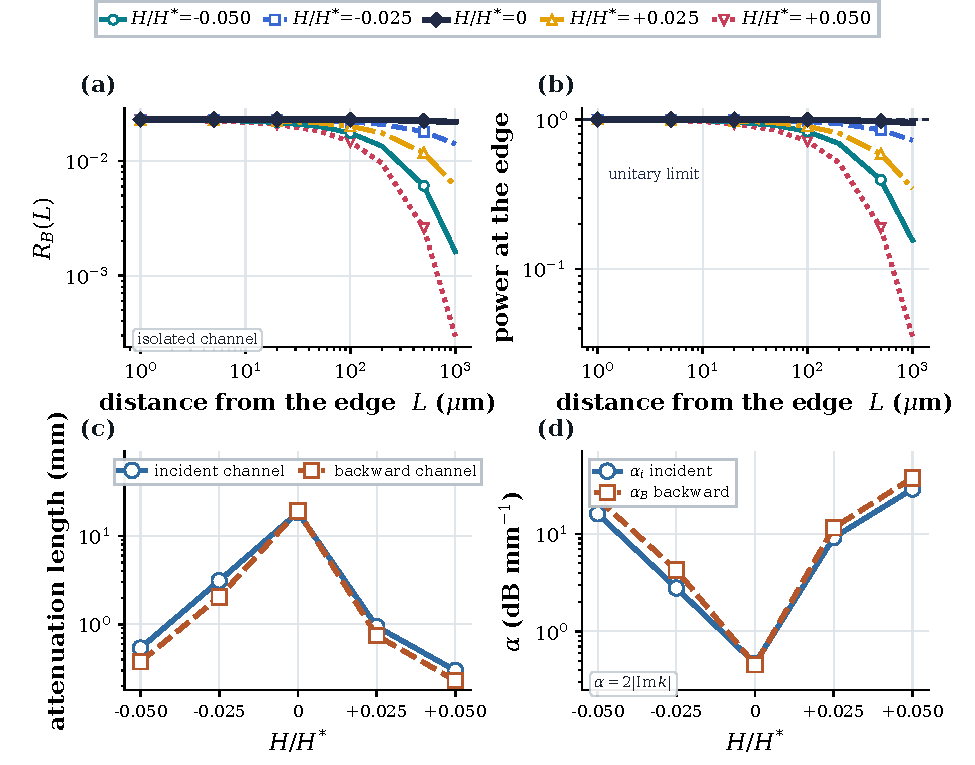
\includegraphics[width=0.95\textwidth]{figures/fig06_attenuation.pdf}
\caption{Distance, survival and attenuation.  (a) Backward channel against the
distance from the edge, isolated-channel convention; (b) incident power arriving
at the edge, normalised to its edge value, with the unitary limit marked;
(c) attenuation length $L$ and (d) loss coefficient $\alpha$, both from the
solved complex spatial roots, against $H/H^{*}$.}
\label{fig:fig06}
\end{figure}

\subsection{Coupling sensitivity in $(k_y,H)$}
\label{sec:results_coupling}

\Cref{fig:fig07} resolves the two-parameter dependence.  Over the solved box
$0.05\le k_yd\le0.20$ and $-0.05\le H/H^{*}\le0.05$, the backward channel ranges
from $0.01896$ to $0.02560$.  Panel (a) shows that the transverse wavenumber
alone accounts for almost all of that range: the five coupling curves are
displaced but their common slope is set by $k_y$.  Panels (c) and (d) quantify
the displacement: against $H/H^{*}$ at fixed operating frequency the relative
change is at most \SI{2.44}{\percent}, and against $k_y$ it is a slow drift that
never exceeds the same bound.  The ratio of the two sensitivities is the
quantitative statement of this paper about the added coupling: $k_y$ changes the
backward channel by a factor of $1.35$ across the box, while $H$ changes it by
at most \SI{2.4}{\percent} at fixed frequency and by \SI{1.21}{\percent} in the
branch-consistent comparison of \cref{tab:controls}.  The coupling is a
perturbation of the partition and not its organising parameter.  The comparison
must be made at fixed $k_x$, because it is the branch and not the coupling that
organises the partition; the two sensitivities do meet, however, at the branch
maximum, where the branch-consistent coupling effect grows to
\SI{34.2}{\percent} (\cref{tab:controls}) while the $k_y$ factor stays at
$1.35$.

Panel (b) draws the measured $5\times19$ grid cell by cell, with no
interpolation beyond the computational box and no smoothing between the five
coupling levels.  Every row of the grid satisfies \eqref{eq:admissible}.

\begin{figure}[htbp]
\centering
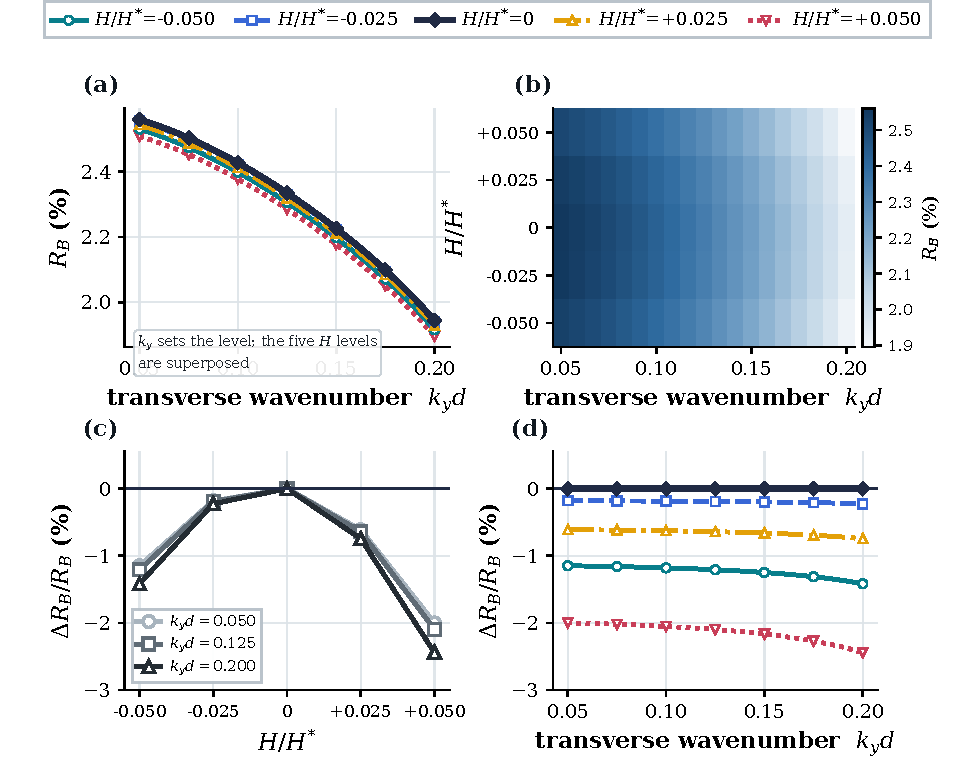
\includegraphics[width=0.95\textwidth]{figures/fig07_coupling.pdf}
\caption{Coupling sensitivity in the $(k_y,H)$ plane.  (a) Backward channel
against $k_yd$ for five $H/H^{*}$; (b) the measured $R_B(k_yd,H)$ grid, drawn
without interpolation; (c) relative change against $H/H^{*}$ along three
declared $k_yd$ slices; (d) the same relative change against $k_yd$.}
\label{fig:fig07}
\end{figure}

\subsection{Through-thickness flux distribution}
\label{sec:results_boundary}

\Cref{fig:fig08} examines how the backward flux is distributed through the
thickness.  The plotted quantity is the $x$ component of the backward Poynting
flux, normalised by the incident flux, as a function of $z/d$; it is an
evaluated field, not an interpolated surface.

The distribution is a signature of the mode rather than of the edge.  The $x$ component
changes sign inside the plate --- it is positive near both free surfaces and
negative in the core, reaching $-0.0367$ and $+0.0317$ in normalised units ---
while its thickness integral remains negative.  The net backward power is
therefore carried by a mode whose local flux direction alternates across the
thickness, which is a property of the strain-gradient plate mode and not of the
edge.  The $z$ component behaves differently: it is largest at the free
surfaces and does not vanish there, so the surfaces carry a transverse flux even
though both traction and double traction vanish on them.  That is exactly the
configuration in which the reactive near field must be retained at the edge
plane, and the reason why \cref{fig:fig05} separates the reactive content from
the transported content instead of adding them.

Panel (c) gives the running thickness integral normalised to its own total, so
the curve rises from zero to one across the plate for every coupling level and
the five curves are indistinguishable.  Panel (d) compares the shape of the
backward and incident $x$ fluxes at $H=0$, both normalised by their own maxima;
the backward mode is more strongly concentrated towards one face than the
incident one.

\begin{figure}[htbp]
\centering
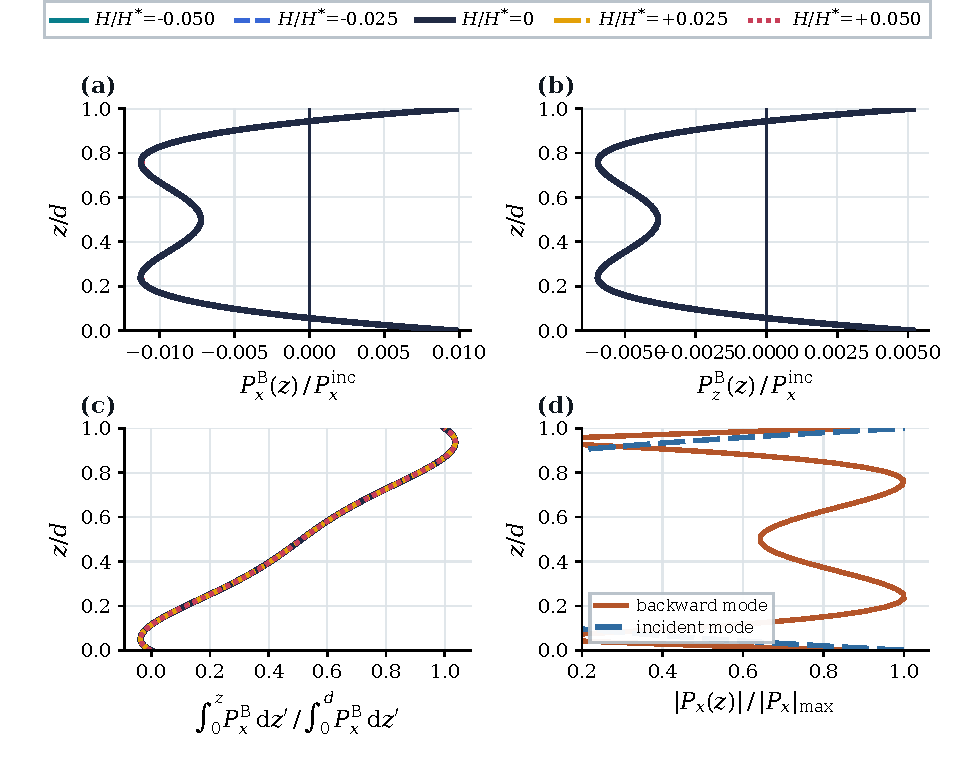
\includegraphics[width=0.95\textwidth]{figures/fig08_boundary.pdf}
\caption{Through-thickness distribution of the backward flux at the reference
plane.  (a) $P_x^{\mathrm{B}}(z)$ and (b) $P_z^{\mathrm{B}}(z)$ normalised by
the incident flux, for five $H/H^{*}$; (c) running thickness integral of
$P_x^{\mathrm{B}}$ normalised to its own total; (d) shape comparison between the
backward and incident $x$ fluxes.  These are normalised profiles; the local flux is reported as computed and is
not independently validated.}
\label{fig:fig08}
\end{figure}

\subsection{Convergence and cross-checks}
\label{sec:results_validation}

\Cref{fig:fig09} documents the numerical behaviour of the edge solve.  Panels
(a) and (b) show the relative error of the backward channel and of the backward
wavenumber against the degree-30 reference: the channel error falls from
$3\times10^{-6}$ at $n=14$ to $10^{-7}$ at $n=26$, while the wavenumber error
stays at the $10^{-12}$ round-off floor over the whole range, so the channel
error is still decreasing at the highest degree used for production.  Panel (c)
shows the scaled edge residual and the relative energy-balance error for every
degree: the residual stays at $3\times10^{-15}$ and the energy-balance error
between $2\times10^{-13}$ and $1\times10^{-12}$, six to seven orders below the
$10^{-8}$ tolerance and two to three orders below the $10^{-10}$ tolerance drawn
in the panel.  Panel (d) compares the temporal and spatial routes for the same
dispersion relation across the box; they agree to $2\times10^{-5}$.

The last panel is a check on the implementation, not a physical validation.  The
two routes discretise the same variational statement and differ only in which
variable is used as the eigenvalue; agreement to $2\times10^{-5}$ shows that the
assembly, the boundary conditions and the elimination of the potential are
implemented consistently.  The independent checks are the strong-form
integrations and the $C^1$ finite-element plate of
\cref{sec:numerics_verification}, neither of which shares the spectral matrices
with the production path.

\begin{figure}[htbp]
\centering
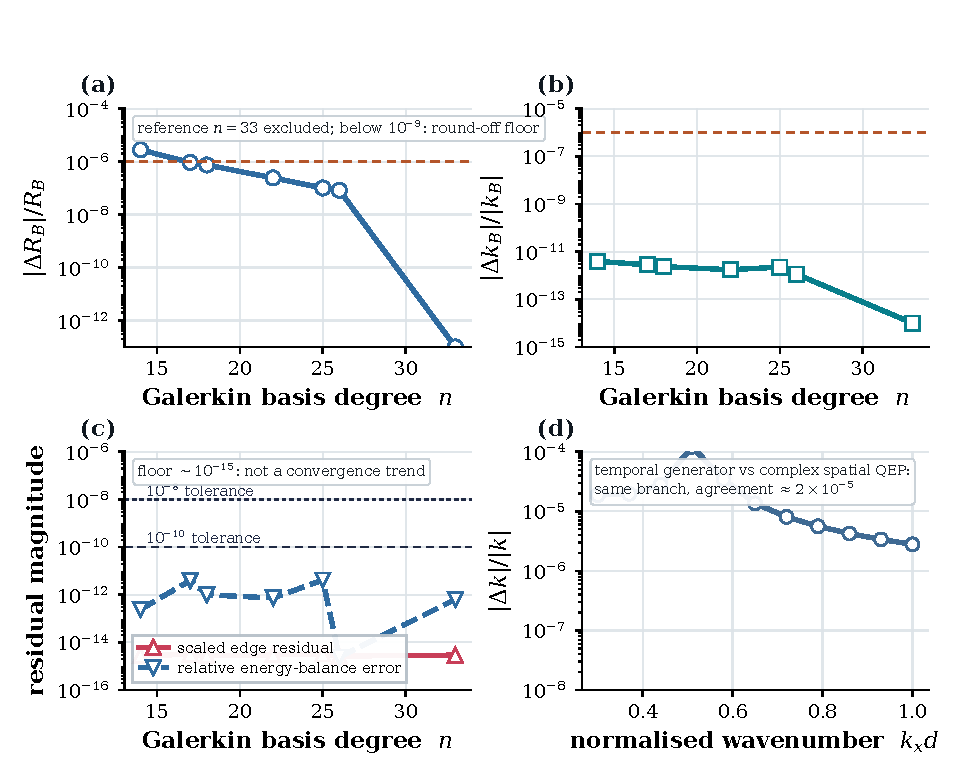
\includegraphics[width=0.95\textwidth]{figures/fig09_validation.pdf}
\caption{Convergence and cross-checks.  (a) Relative error of the backward
channel and (b) of the backward wavenumber against the Galerkin degree, with the
degree-30 reference; (c) scaled edge residual and relative energy-balance error
with the tolerance lines; (d) relative difference between the temporal-generator
and the spatial eigenvalue routes, which is a consistency check of the
implementation and not an independent physical validation.}
\label{fig:fig09}
\end{figure}

\subsection{Wave field and flux directions}
\label{sec:results_field}

\Cref{fig:fig10} closes the presentation with the solved field.  Panels (a) and
(b) show the incident and backward intensities on a shared logarithmic colour
scale over $x\in[-60,1.5]\,\si{\micro\metre}$ and
$y\in[-45,45]\,\si{\micro\metre}$; the vertical line at $x=0$ is the edge, the
plate lies to its left, and the intensities are normalised to a common maximum
so that the backward field is visibly weaker by one to three decades.  The
incident field approaches the edge at $+10.0^{\circ}$ and the backward field
leaves it at $-27.9^{\circ}$, both measured from the thickness-integrated
Poynting flux.

Panel (c) is a schematic, but its arrows are not drawn by hand: they are the
solved directions, $\vect{k}_i\propto(1,0.176)$, $\vect{k}_B\propto(0.333,-0.530)$,
$\vect{P}_i\propto(1,0.176)$ and $\vect{P}_B\propto(-1,-0.530)$, taken from the
computed flux of the incident and backward modes.  The last of these is the
geometric content of the word ``negative'': the backward mode carries energy in
$-x$ and in $-y$ simultaneously, so its energy transport is opposite in both
components to that of the incident wave.  Panel (d) shows the two components of
the backward flux against $k_yd$; both are negative throughout the box, and both
tend to a common small value as $k_yd\to0.2$.

\begin{figure}[htbp]
\centering
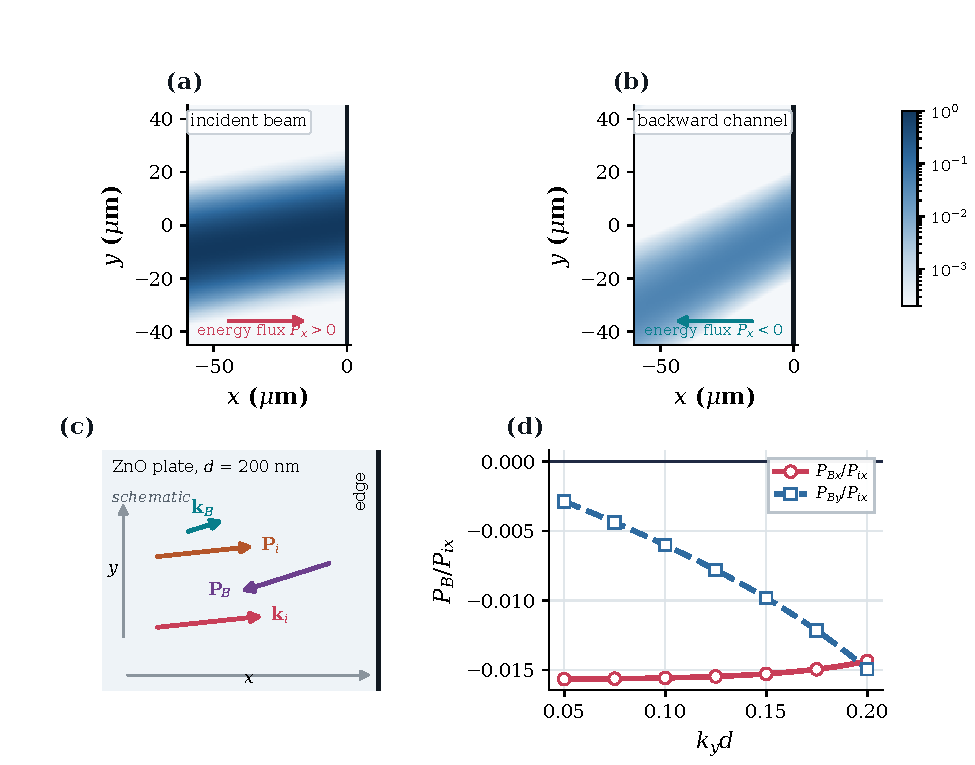
\includegraphics[width=0.95\textwidth]{figures/fig10_field.pdf}
\caption{Solved field maps and flux directions.  (a) Incident and (b) backward
intensity on a shared logarithmic scale, with the edge at $x=0$; (c) schematic
whose arrows are the solved flux directions of the incident and backward modes;
(d) the two components of the backward flux against $k_yd$.}
\label{fig:fig10}
\end{figure}
